\section{Estado de avance}

Para comenzar el desarrollo de ChiVO fue necesario identificar aparte de los
requerimientos y casos de uso, las interacciones que los usuarios realizarán
con el sistema. El diagrama de secuencia de interacción entre el usuario y
ChiVO se puede ver en la figura \ref{fig:secuencia}.
En base a este diagrama, requerimientos y tecnologías utilizadas el estado de
avance se especificará por cada capa de abstracción.

\begin{figure*}[h!t]
    \centering
    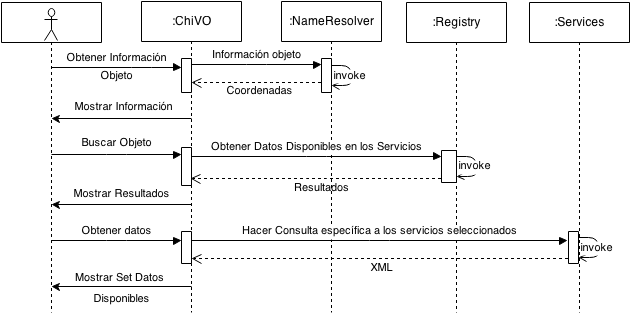
\includegraphics[width=0.7\textwidth]{images/secuencia.png}
    \caption{Diagrama de secuencia entre Usuario y ChiVO}
    \label{fig:secuencia}
\end{figure*}

La arquitectura de software de ChiVO está basada en el uso de protocolos y estándares de
IVOA. Estos protocolos y estándares están agrupados en capas, de las cuales
destacamos la capa de aplicación y la de datos (ver Figura~\ref{fig:ivoarch}),
ya que sus estándares básicos definen la operación mínima que un VO debe
realizar. A continuación, se detallan los elementos que ChiVO ha implementado
en estas capas.
\begin{figure}[ht]
    \centering
    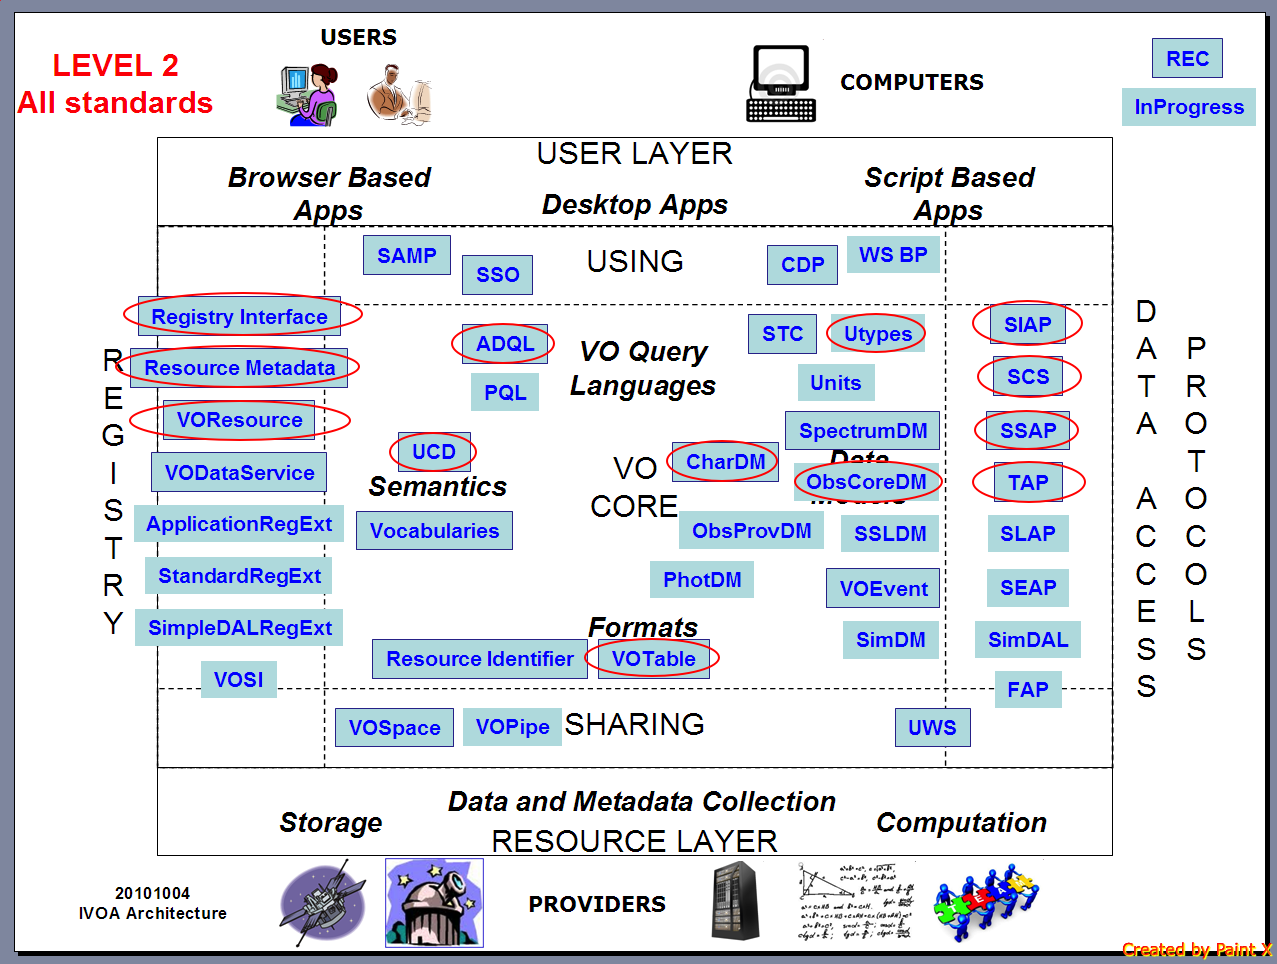
\includegraphics[width=0.45\textwidth]{images/arquitectura_2.png}
    \caption{Arquitectura de IVOA con los Protocolos y Estándares usados}
    \label{fig:ivoarch}
\end{figure}

\begin{description}
    \item[Capa Aplicación:] \hfill \\
        Un Servicio Web compatible con VO necesita al menos un \emph{Table Access
        Protocol} para acceder al modelo de datos de ChiVO usando el
        \emph{Astronomical Data Query Language}.
        Además, para el cumplimiento de los requerimientos del sistema,
        actualmente se ha implementado
        el protocolo para realizar búsquedas cónicas \emph{Simple Cone Search}, el protocolo para realizar acceder a datos
        espectrales \emph{Simple Spectral Access} y el protocolo de
        acceso a imágenes \emph{Simple Image Access}.

    \item[Capa de datos:] \hfill \\
        En esta capa se requiere la configuración de la base de datos relacional con
        un modelo de datos recomendado por IVOA llamado \emph{Observation Core Data
        Model}. Este modelo de datos permite que los VO sean interoperables,
        ya que definen una cantidad mínima de atributos en las tablas con cierto
        nombre y tipo de dato, de forma que acceder a diferentes servicios mediante
        \emph{TAP + Obscore} es estándar.
        Además el formato de transferencia de información (metadata) es con el
        formato estándar \emph{XML VOTable}.
\end{description}

\subsection{Capa de abstracción: Clientes}

Dento del diagrama de secuencia, el Frontend es el VO-Client, es decir, está a cargo
de generar la interacción entre los usuarios y los demás elementos dentro del
sistema.

Actualmente se generó un frontend en RoR que permite interactuar con:

\begin{description}
    \item[Resolver nombres]:\hfill \\
        a partir de un nombre (String) retorna la posición de un objeto en
        coordenadas celestiales usando el servicio SESAME de Astrogrid.
    \item[Registro]: \hfill \\
        busca servicios dentro del endpoint, y luego según lo que necesite el
        usuario elige sobre cuales trabajar para hacer consultas.
    \item[Servicios]: \hfill \\
        consulta a diferentes servicios web que proveen datos mediante cierto
        protocolo y unifica los resultados en un XML VOTable para ser desplegados
        en forma ordenada usando una biblioteca de javascript VOView.
\end{description}

\subsection{Capa de abstracción: Aplicaciones}

El Endpoint está a cargo de generar una interacción transparente entre los clientes
de VO y los posibles recursos que se configuren.
En este caso el Endpoint genera una interfaz para los servicios configurados por el
Backend y los disponibles a través del registro de VO-Paris.
VO-Paris posee una Web API en REST que permite consultar por recursos y retorna un
archivo JSON con resultados.

\subsection{Capa de abstracción: Datos}

Actualmente ALMA le facilita a ChiVO datos públicos, los cuales incluyen ASDM,
Measurement \cite{petry2012analysing}, FITS \cite{wells1981fits}, de los cuales es
necesario extraer los metadatos del ObsCoreDM para ser ingresados a la base de datos.

\begin{figure}[h!t]
    \centering
    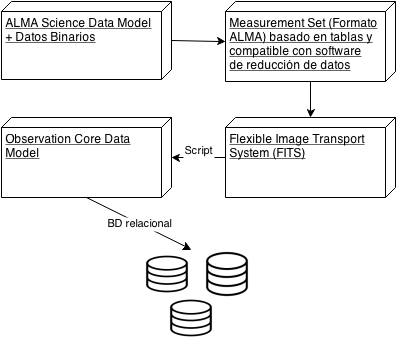
\includegraphics[width=0.45\textwidth]{images/metadata.png}
    \caption{Proceso transformación desde Frontend de ALMA hasta la base de datos
             de ChiVO}
    \label{fig:metadata}
\end{figure}

El procedimiento se hace a través de un programa, el cual usando el framework de
backend DaCHS \cite{dachs}, permite configurar recursos y servicios mediante
archivos de configuración Resource Descriptor \cite{dachsorguide}.
Una vez creadas las entradas en la base de datos y configurados los servicios SCS,
SSAP, SIAP, TAP se pueden acceder mediante las consultas definidas en cada
protocolo.

